% Relaxation dispersion.
%%%%%%%%%%%%%%%%%%%%%%%%

\chapter[Relaxation dispersion]{The analysis of relaxation dispersion} \label{ch: relax-disp}
\index{relaxation dispersion|textbf}

\begin{figure*}[h]
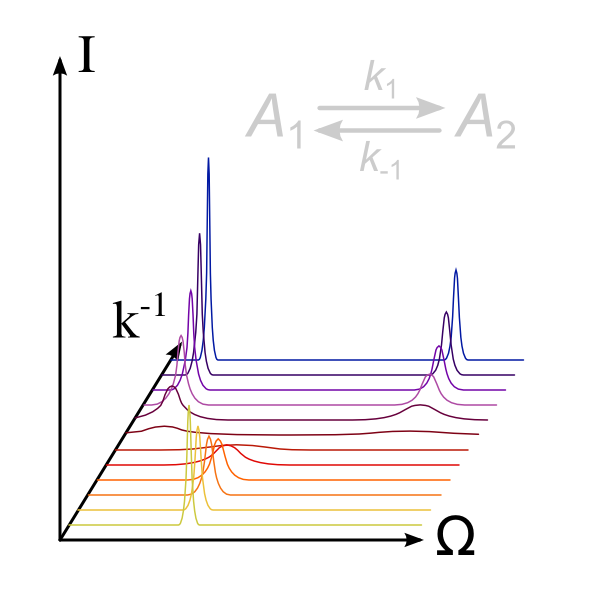
\includegraphics[width=5cm, bb=0 0 1701 1701]{graphics/analyses/relax_disp_600x600}
\end{figure*}


% Introduction.
%%%%%%%%%%%%%%%

\section{Introduction to relaxation dispersion}

Relaxation dispersion is the experimental modulation of chemical exchange relaxation.  For the $\Ronerho$-type experiment in which the nucleus of interest is spin-locked, either the spin-lock field strength or the offset between the spin-lock pulse and the chemical shift of the spins is used to modulate the exchange.  For the CPMG-type experiment, varying the time between the pulses modules the exchange.  Both experiment types are handled by relax.


% The models.
%%%%%%%%%%%%%

\section{The modelling of dispersion data}

For a system under the influence of chemical exchange, the evolution of the transverse magnetisation is given by the \citet{Bloch46} equations as modified by \citet{McConnell58} for chemical exchange -- the Bloch-McConnell equations.
For a two state exchange jumping between states A and B, the equation is:

\begin{equation} \label{eq: Bloch-McConnell}
    \frac{d}{dt} \left[ 
        \begin{array}{c}
            M_A^+(t) \\
            M_B^+(t)
        \end{array}
    \right] = \left[
        \begin{array}{cc}
            -i\Omega_A-\RtwozeroA-\pB\kex & \pA\kex \\
            \pB\kex & -i\Omega_B-\RtwozeroB-\pA\kex \\
        \end{array}
    \right] \left[
        \begin{array}{c}
            M_A^+(t) \\
            M_B^+(t)
        \end{array}
    \right] .
\end{equation}

The solution to this equation then Fourier transformed to produce the NMR spectrum.  However the analytic or closed-form frequency-domain solution remains intractable.

Solutions can nevertheless be found by either making assumptions or restrictions about the exchange process and then analytically solving~\ref{eq: Bloch-McConnell} or by numerical simulation.
The modelling of relaxation dispersion data can hence be catergorised into these two distinct methodologies:

\begin{description}
\item[Analytical models:]\index{relaxation dispersion!Analytical model}  Optimisation of models based on analytical, closed-form expressions derived from the Bloch-McConnell equations subject to certain conditions (see Section~\ref{sect: dispersion: analytic models} on page~\pageref{sect: dispersion: analytic models}).
\item[Numerical models:]\index{relaxation dispersion!Numerical model}  Optimisation of models based on numerically solving the Bloch-McConnell equations (see Section~\ref{sect: dispersion: numerical models} on page~\pageref{sect: dispersion: numerical models}).
\end{description}



% Analytic models.
%~~~~~~~~~~~~~~~~~

\subsection{Analytic models}
\label{sect: dispersion: analytic models}
\index{relaxation dispersion!Analytical model|textbf}

A number of analytic models are supported within relax.
If the model you are interested in is not available, see Section~\ref{sect: dispersion: model tutorial} on page~\pageref{sect: dispersion: model tutorial} for how new models can be added to relax.
The analytic models are dependant upon whether the data originates from a CPMG-type or $\Ronerho$-type experiment.
For the CPMG-type experiments, the models currently supported are:

\begin{description}
\item[`R2eff':]\index{relaxation dispersion!R2eff model}  This is the model used to determine the $\Rtwoeff$ values and errors required as the base data for all other models.  See Section~\ref{sect: dispersion: R2eff model} on page~\pageref{sect: dispersion: R2eff model}.
\item[`No Rex':]\index{relaxation dispersion!No Rex model}  This is the model for no chemical exchange being present.  See Section~\ref{sect: dispersion: No Rex model} on page~\pageref{sect: dispersion: No Rex model}.
\item[`LM63':]\index{relaxation dispersion!LM63 model}  The original \citet{LuzMeiboom63} 2-site fast exchange equation with parameters $\{\Rtwozero, \dots, \Phiex, \kex\}$.  See Section~\ref{sect: dispersion: LM63 model} on page~\pageref{sect: dispersion: LM63 model}.
\item[`CR72 red':]\index{relaxation dispersion!CR72 red model}  The \citet{CarverRichards72} 2-site equation for all time scales whereby the simplification $\RtwozeroA = \RtwozeroB$ is assumed.  It has the parameters $\{\Rtwozero, \dots, \pA, \dw, \kex\}$.  See Section~\ref{sect: dispersion: CR72 red model} on page~\pageref{sect: dispersion: CR72 red model}.
\item[`CR72':]\index{relaxation dispersion!CR72 model}  The \citet{CarverRichards72} 2-site equation for all time scales with parameters $\{\RtwozeroA, \RtwozeroB, \dots, \pA, \dw, \kex\}$.  See Section~\ref{sect: dispersion: CR72 model} on page~\pageref{sect: dispersion: CR72 model}.
\item[`IT99':]\index{relaxation dispersion!IT99 model}  The \citet{IshimaTorchia99} 2-site model for all time scales with $\pA \gg \pB$ and with parameters $\{\Rtwozero, \dots, \Phiex, \pA.\dw^2, \kex\}$.  See Section~\ref{sect: dispersion: IT99 model} on page~\pageref{sect: dispersion: IT99 model}.
\end{description}

For the $\Ronerho$-type experiment, the currently supported models are:

\begin{description}
\item[`R2eff':]\index{relaxation dispersion!R2eff model}  This is the same model model as for the CPMG-type experiments except that the $\Ronerho$ and not $\Rtwoeff$ values are determined.  See Section~\ref{sect: dispersion: R2eff model} on page~\pageref{sect: dispersion: R2eff model}.
\item[`No Rex':]\index{relaxation dispersion!No Rex model}  This is the model for no chemical exchange being present.  See Section~\ref{sect: dispersion: No Rex model} on page~\pageref{sect: dispersion: No Rex model}.
\item[`M61':]\index{relaxation dispersion!M61 model}  The \citet{Meiboom61} 2-site fast exchange equation for on-resonance data with parameters $\{\Ronerhoprime, \dots, \Phiex, \kex\}$.  See Section~\ref{sect: dispersion: M61 model} on page~\pageref{sect: dispersion: M61 model}.
\item[`DPL94':]\index{relaxation dispersion!DPL94 model}  The \citet{Davis94} 2-site fast exchange equation for off-resonance data with parameters $\{\Ronerhoprime, \dots, \Phiex, \kex\}$.  See Section~\ref{sect: dispersion: DPL94 model} on page~\pageref{sect: dispersion: DPL94 model}.
\item[`M61 skew':]\index{relaxation dispersion!M61 skew model}  The \citet{Meiboom61} 2-site equation for all time scales with $\pA \gg \pB$ and with parameters $\{\Ronerhoprime, \dots, \pA, \dw, \kex\}$.  This model is disabled by default in the dispersion auto-analysis.  See Section~\ref{sect: dispersion: M61 skew model} on page~\pageref{sect: dispersion: M61 skew model}.
\end{description}



% Numerical models.
%~~~~~~~~~~~~~~~~~~

\subsection{Numerical models}
\label{sect: dispersion: numerical models}
\index{relaxation dispersion!Numerical model|textbf}

Like the analytic models, a number of numerical models are supported within relax.
These models are also dependant upon whether the data originates from a CPMG-type or $\Ronerho$-type experiment.
For the CPMG-type experiments, the models currently supported are:

\begin{description}
\item[`R2eff':]\index{relaxation dispersion!R2eff model}  This is the model used to determine the $\Rtwoeff$ values and errors required as the base data for all other models.  See Section~\ref{sect: dispersion: R2eff model} on page~\pageref{sect: dispersion: R2eff model}.
\item[`No Rex':]\index{relaxation dispersion!No Rex model}  This is the model for no chemical exchange being present.  See Section~\ref{sect: dispersion: No Rex model} on page~\pageref{sect: dispersion: No Rex model}.
\item[`NS 2-site star red':]\index{relaxation dispersion!NS 2-site star red model}  A model for 2-site exchange using complex conjugate matrices whereby the simplification $\RtwozeroA = \RtwozeroB$ is assumed.  It has the parameters $\{\Rtwozero, \dots, \pA, \dw, \kex\}$.  See Section~\ref{sect: dispersion: NS 2-site star red model} on page~\pageref{sect: dispersion: NS 2-site star red model}.
\item[`NS 2-site star':]\index{relaxation dispersion!NS 2-site star model}  A model for 2-site exchange using complex conjugate matrices with parameters $\{\RtwozeroA, \RtwozeroB, \dots, \pA, \dw, \kex\}$.  See Section~\ref{sect: dispersion: NS 2-site star model} on page~\pageref{sect: dispersion: NS 2-site star model}.
\end{description}


For the $\Ronerho$-type experiment, only the base models are currently supported:

\begin{description}
\item[`R2eff':]\index{relaxation dispersion!R2eff model}  This is the model used to determine the $\Rtwoeff$ values and errors required as the base data for all other models.  See Section~\ref{sect: dispersion: R2eff model} on page~\pageref{sect: dispersion: R2eff model}.
\item[`No Rex':]\index{relaxation dispersion!No Rex model}  This is the model for no chemical exchange being present.  See Section~\ref{sect: dispersion: No Rex model} on page~\pageref{sect: dispersion: No Rex model}.
\end{description}





% Dispersion model summary.
%~~~~~~~~~~~~~~~~~~~~~~~~~~

\subsection{Dispersion model summary}

Except for `R2eff' and `No Rex', all models can be fit to clusterings of spins, or spin blocks.
The models are described in more detail below and summarised in Table~\ref{table: CPMG dispersion models} for CPMG-type experiments and Table~\ref{table: R1rho dispersion models} for $\Ronerho$-type experiments.
The parameters are given in Table~\ref{table: dispersion parameters}.

\begin{sidewaystable}
\begin{center}
\caption{The parameters of relaxation dispersion.}
\begin{tabular}{llll}
\toprule
Parameter               & Equation              & Description                                                                   & Units \\
\midrule
$\nucpmg$               & $1 / (2 \taucpmg)$    & CPMG frequency                                                                & Hz \\
$\taucpmg$              & $1 / (2 \nucpmg)$     & Delay between CPMG $\pi$ pulses                                               & s \\
$T_\textrm{relax}$      & -                     & The relaxation delay period                                                   & s \\
$I_0$                   & -                     & Reference peak intensity when $T_\textrm{relax}$ is zero                      & - \\
$I_1$                   & -                     & Peak intensity for a given $\nucpmg$ or spin-lock field strength $\omega_1$   & - \\
$\Rtwozero$             & -                     & $\Rtwo$ relaxation rate in the absence of exchange                            & rad.s$^{-1}$ \\
$\RtwozeroA$            & -                     & $\Rtwo$ relaxation rate for state A in the absence of exchange                & rad.s$^{-1}$ \\
$\RtwozeroB$            & -                     & $\Rtwo$ relaxation rate for state B in the absence of exchange                & rad.s$^{-1}$ \\
$\Ronerhoprime$         & -                     & $\Ronerho$ relaxation rate in the absence of exchange                         & rad.s$^{-1}$ \\
$\theta$                & -                     & Rotating frame tilt angle                                                     & rad \\
$\omegaone$             & -                     & Spin-lock field strength                                                      & rad.s$^{-1}$ \\
$\omegae$               & -                     & Effective field in the rotating frame                                         & rad.s$^{-1}$ \\
$\kex$                  & $1 / (2 \tex)$        & Chemical exchange rate constant                                               & rad.s$^{-1}$ \\
$\tex$                  & $1 / (2 \kex)$        & Time of exchange                                                              & s.rad$^{-1}$ \\
$\pA$                   & -                     & Population of state A                                                         & - \\
$\pB$                   & -                     & Population of state B                                                         & - \\
$\dw$                   & -                     & Chemical shift difference between the two states                              & ppm \\
$\Phiex$                & $\pA\pB\dw^2$         & Fast exchange factor                                                          & rad$^2$.s$^{-2}$ \\
\bottomrule
\label{table: dispersion parameters}
\end{tabular}
\end{center}
\end{sidewaystable}


\begin{sidewaystable}
\begin{center}
\caption{The analytic and numerical models for CPMG-type experiments currently supported within relax}
\begin{tabular}{lllcll}
\toprule
Model code         & Type     & Sites & Parameters                                          & Restriction                       & Reference \\
\midrule                              
R2eff              & -        & -     & $\{\Rtwoeff, \cdots\}$                              & Fixed relaxation time period      & - \\
R2eff              & -        & -     & $\{\Rtwoeff, I_0, \cdots\}$                         & Variable relaxation time period   & - \\
No Rex             & -        & 0     & $\{\Rtwozero, \cdots\}$                             & -                                 & - \\
LM63               & Analytic & 2     & $\{\Rtwozero, \dots, \Phiex, \kex\}$                & Fast exchange                     & \citet{LuzMeiboom63} \\
CR72 red           & Analytic & 2     & $\{\Rtwozero, \dots, \pA, \dw, \kex\}$              & $\pA > \pB$                       & \citet{CarverRichards72} \\
CR72               & Analytic & 2     & $\{\RtwozeroA, \RtwozeroB, \dots, \pA, \dw, \kex\}$ & $\pA > \pB$                       & \citet{CarverRichards72} \\
IT99               & Analytic & 2     & $\{\Rtwozero, \dots, \Phiex, \pA.\dw^2, \kex\}$     & $\pA \gg \pB$                     & \citet{IshimaTorchia99} \\
NS 2-site star red & Numeric  & 2     & $\{\Rtwozero, \dots, \pA, \dw, \kex\}$              & $\pA > \pB$                       & - \\
NS 2-site star     & Numeric  & 2     & $\{\RtwozeroA, \RtwozeroB, \dots, \pA, \dw, \kex\}$ & $\pA > \pB$                       & - \\
\bottomrule
\label{table: CPMG dispersion models}
\end{tabular}
\end{center}
\end{sidewaystable}


\begin{sidewaystable}
\begin{center}
\caption{The analytic and numerical models for $\Ronerho$-type experiments currently supported within relax.}
\begin{tabular}{lllcll}
\toprule
Model code & Type     & Sites & Parameters                                        & Restriction                       & Reference \\
\midrule                       
R2eff      & -        & -     & $\{\Ronerho, \cdots\}$                            & Fixed relaxation time period      & - \\
R2eff      & -        & -     & $\{\Ronerho, I_0, \cdots\}$                       & Variable relaxation time period   & - \\
No Rex     & -        & 0     & $\{\Ronerhoprime, \cdots\}$                       & -                                 & - \\
M61        & Analytic & 2     & $\{\Ronerhoprime, \dots, \Phiex, \kex\}$          & Fast exchange, on-resonance       & \citet{Meiboom61} \\
DPL94      & Analytic & 2     & $\{\Ronerhoprime, \dots, \Phiex, \kex\}$          & Fast exchange                     & \citet{Davis94} \\
M61 skew   & Analytic & 2     & $\{\Ronerhoprime, \dots, \pA, \dw, \kex\}$        & $\pA \gg \pB$, on-resonance       & \citet{Meiboom61} \\
\bottomrule
\label{table: R1rho dispersion models}
\end{tabular}
\end{center}
\end{sidewaystable}


% R2eff model.
%~~~~~~~~~~~~~

\clearpage

\subsection{The R2eff model}
\label{sect: dispersion: R2eff model}
\index{relaxation dispersion!R2eff model|textbf}

This is the simplest of all models in that the dispersion component of the base data -- the peak intensity values -- is not modelled.  It is used to determine either the $\Rtwoeff$ or $\Ronerho$ values and errors as required for the base data for all other models.  It can be selected by setting the model to `R2eff'.  Depending on the experiment type, this model will be handled differently.  The $\Rtwoeff$/$\Ronerho$ values determined can be later copied to the data pipes of the other dispersion models using the appropriate user functions.


% Fixed relaxation period experiments.
\subsubsection{Fixed relaxation period experiments}

For the fixed relaxation time period CPMG-type experiments, the $\Rtwoeff$/$\Ronerho$ values are determined by direct calculation using the formula
\begin{equation}
    R_{2\textrm{eff}}(\nucpmg) = - \frac{1}{T_\textrm{relax}} \cdot \ln \left( \frac{I_1(\nucpmg)}{I_0} \right) .
\end{equation}

The values and errors are determined with a single call of the \uf{calc} user function.  The $\Ronerho$ version of the equation is essentially the same:
\begin{equation}
    R_{1\rho}(\omega_1) = - \frac{1}{T_\textrm{relax}} \cdot \ln \left( \frac{I_1(\omega_1)}{I_0} \right) .
\end{equation}

Errors are calculated using the formula
\begin{equation} \label{eq: dispersion error}
    \sigma_{\textrm{R}_2} = \frac{1}{T_\textrm{relax}} \sqrt{ \left( \frac{\sigma_{I_1}}{I_1(\omega_1)} \right)^2  +  \left( \frac{\sigma_{I_0}}{I_0} \right)^2 } .
\end{equation}

In a number of publications, the error formula from \citet{IshimaTorchia05} has been used.  This is the collapse of Equation~\ref{eq: dispersion error} by setting $\sigma_{I_0}$ to zero:
\begin{equation} \label{eq: IT05 dispersion error}
    \sigma_{\textrm{R}_2} = \frac{\sigma_{I_1}}{T_\textrm{relax} I_1(\omega_1)} .
\end{equation}

This is not implemented in relax as it can be shown by simple simulation that the formula is incorrect (see Figure~\ref{fig: dispersion error comparison}).  This formula significantly underestimates the real errors.  The use of the same $I_0$ value for all dispersion points does not cause a decrease in the $\Rtwoeff$ error but rather a correlation in the errors.

\begin{figure*}[h]
\label{fig: dispersion error comparison}
\centerline{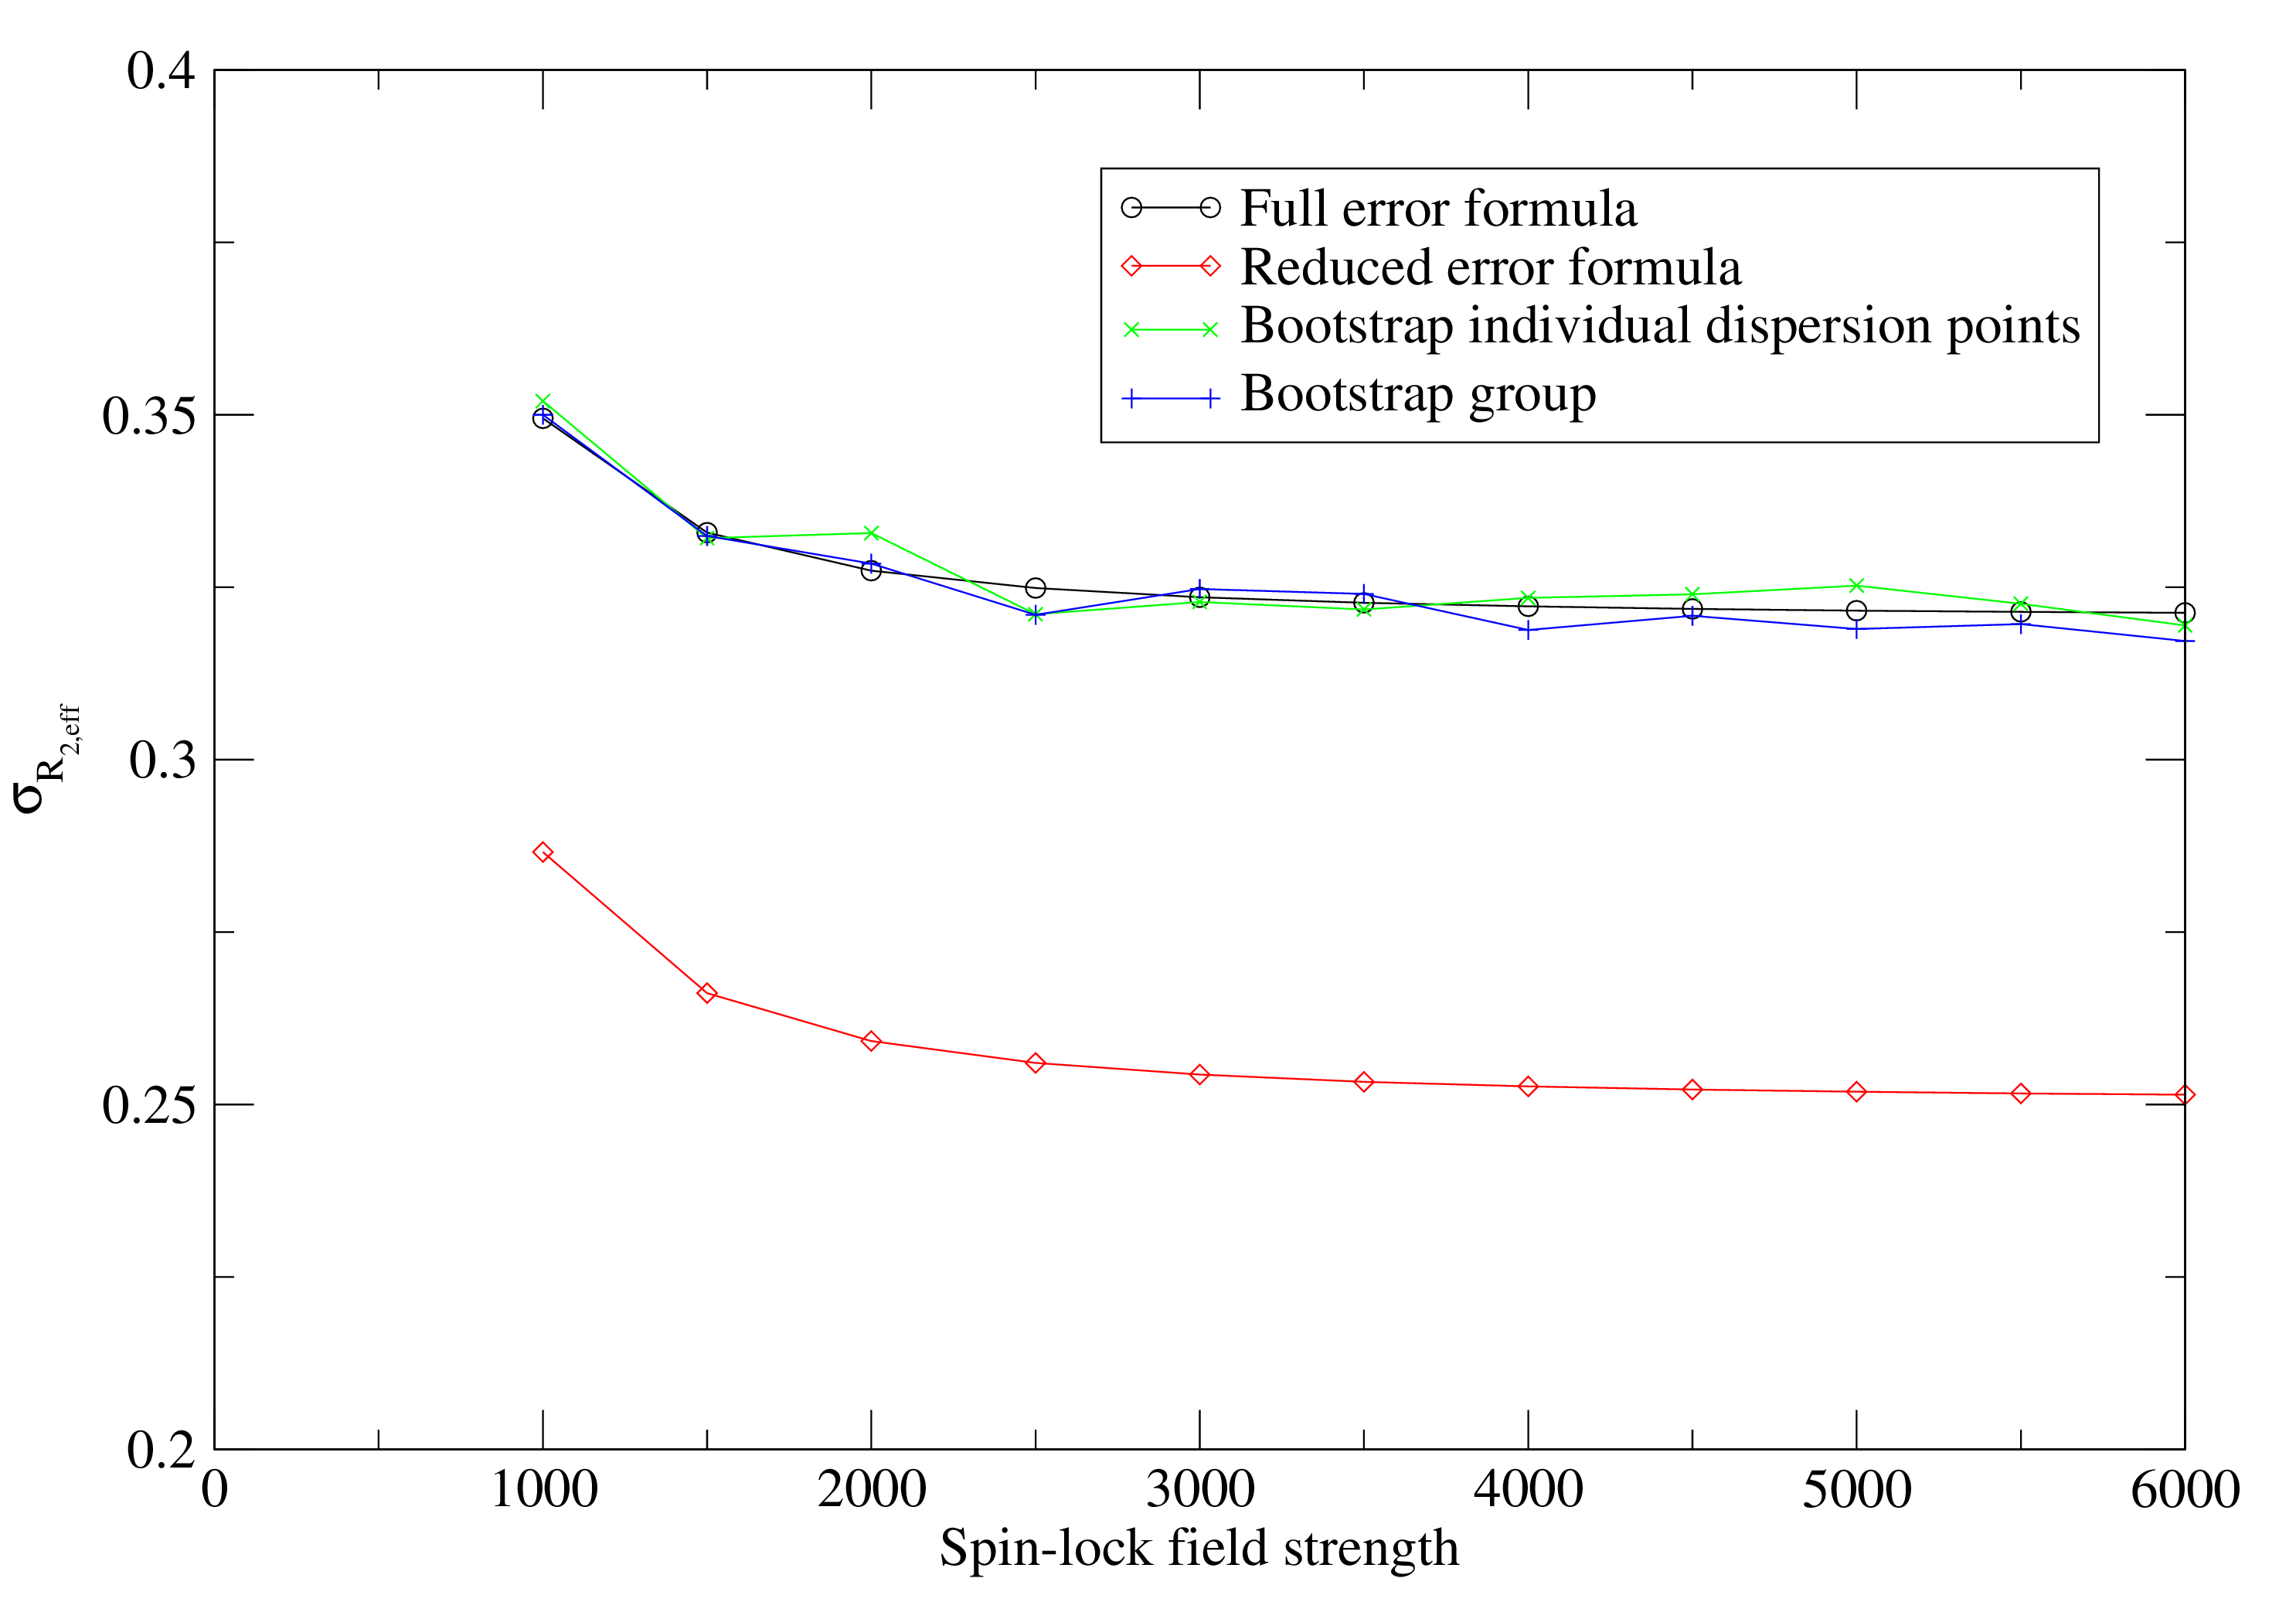
\includegraphics[width=0.9\textwidth, bb=14 14 728 512]{graphics/analyses/dispersion/error_comparison}}
\caption[Comparison of relaxation dispersion errors]{A demonstration of the inaccuracy of the error formula of Equation~\ref{eq: IT05 dispersion error} from \citet{IshimaTorchia05}.  This plot was generated using the script \file{test\_suite/shared\_data/dispersion/error\_testing/simulation.py}.  The bootstrapping simulation involves randomising noise-free $I_0$ and $I_1$ values for each dispersion data point assuming Gaussian errors.  The full error formula is from Equation~\ref{eq: dispersion error}, the reduced error formula is from Equation~\ref{eq: IT05 dispersion error}, the bootstrapping using individual dispersion points estimates the errors assuming different $I_0$ randomisations for each dispersion point and each simulation, and the bootstrapping group graph uses the same randomised $I_0$ value for all dispersion points for each simulation.}
\end{figure*}


% Variable relaxation period experiments.
\subsubsection{Variable relaxation period experiments}

For the variable relaxation time period type experiments, the $\Rtwoeff$/$\Ronerho$ values are determined by fitting to the simple two parameter exponential as in a $\Rone$ or $\Rtwo$ analysis.  Both $\Rtwoeff$/$\Ronerho$ and the initial peak intensity $I_0$ are optimised using the minimise user function for each exponential curve separately.  Monte Carlo simulations are used to obtain the parameter errors.



% No Rex model.
%~~~~~~~~~~~~~~

\subsection{The model for no chemical exchange relaxation}
\label{sect: dispersion: No Rex model}
\index{relaxation dispersion!No Rex model|textbf}

This model is provided for model selection purposes.  In combination with frequentist methods, such as AIC\index{model selection!AIC}, or Bayesian methods\index{model selection!Bayesian} it can show if the presence of chemical exchange is statistically significant.  Optimisation is still required as one $\Rtwozero$ value per magnetic field strength will be fit to the measured data for each spin system.  It is selected by setting the model to `No Rex'.



% LM63 model.
%~~~~~~~~~~~~

\subsection{The LM63 2-site fast exchange CPMG model}
\label{sect: dispersion: LM63 model}
\index{relaxation dispersion!LM63 model|textbf}

This is the original model for 2-site fast exchange for CPMG-type experiments.  It is selected by setting the model to `LM63', here named after \citet{LuzMeiboom63}.  The equation for the exchange process is:
\begin{equation}
    \Rtwoeff = \Rtwozero + \frac{\Phiex}{\kex} \cdot \left( 1 - \frac{4\nucpmg}{\kex} \cdot \tanh \left( \frac{\kex}{4\nucpmg} \right) \right) .
\end{equation}

The reference for this equation is:
\begin{itemize}
\item \bibentry{LuzMeiboom63}
\end{itemize}



% CR72 model.
%~~~~~~~~~~~~

\subsection{The CR72 2-site CPMG model}
\label{sect: dispersion: CR72 model}
\index{relaxation dispersion!CR72 model|textbf}

This is the model for 2-site exchange on all times scales (with the constraint that $\pA > \pB$), named after \citet{CarverRichards72}.  Is it selected by setting the model to `CR72'.  The equation is
\begin{equation}
    \Rtwoeff = \frac{1}{2} \Big( \textrm{R}_\textrm{2A}^0 + \textrm{R}_\textrm{2B}^0 + \kex - 2\nucpmg\cosh^{-1} \big( D_+\cosh(\eta_+) - D_-\cos(\eta_-) \big) \Big) ,
\end{equation}

where
\begin{align}
    D_\pm    &= \frac{1}{2} \left( \pm1 + \frac{\Psi + 2\dw^2}{\sqrt{\Psi^2 + \zeta^2}} \right) , \\
    \eta_\pm &= 2^{\frac{2}{3}}\frac{1}{\nucpmg} \left( \pm\Psi + \sqrt{\Psi^2 + \zeta^2} \right)^{\frac{1}{2}} , \\
    \Psi     &= \left( \textrm{R}_\textrm{2A}^0 - \textrm{R}_\textrm{2B}^0 - \pA\kex + \pB\kex \right)^2 - \dw^2 + 4\pA\pB\kex^2 , \\
    \zeta    &= 2\dw \left( \textrm{R}_\textrm{2A}^0 - \textrm{R}_\textrm{2B}^0 - \pA\kex + \pB\kex \right).
\end{align}

The reference for this equation is:
\begin{itemize}
\item \bibentry{CarverRichards72}
\end{itemize}



% CR72 red model.
%~~~~~~~~~~~~~~~~

\subsection{The CR72 reduced 2-site CPMG model}
\label{sect: dispersion: CR72 red model}
\index{relaxation dispersion!CR72 red model|textbf}

This is the model for 2-site exchange on all times scales (with the constraint that $\pA > \pB$), named after \citet{CarverRichards72}.
Is it selected by setting the model to `CR72 red'.
It is the same as the CR72 model described above, but with the simplification that $\RtwozeroA = \RtwozeroB$.
This simplifies the equations to
\begin{equation}
    \Rtwoeff = \Rtwozero + \frac{\kex}{2} - \nucpmg\cosh^{-1} \big( D_+\cosh(\eta_+) - D_-\cos(\eta_-) \big) ,
\end{equation}

where $D_\pm$ and $\eta_\pm$ are unchanged and
\begin{align}
    \Psi  &= \kex^2 - \dw^2 , \\
    \zeta &= -2\dw (\pA\kex - \pB\kex) .
\end{align}



% IT99 model.
%~~~~~~~~~~~~

\subsection{The IT99 2-site CPMG model}
\label{sect: dispersion: IT99 model}
\index{relaxation dispersion!IT99 model|textbf}

This is the model for 2-site exchange on all times scales (with the constraint that $\pA \gg \pB$), named after Ishima and Torchia 1999.  Is it selected by setting the model to `IT99'.  The equation is:
\begin{align}
    \Rex       &\simeq \frac{\Phiex\tex}{1 + \omega_a^2\tex^2} , \\
    \omega_a^2 &= \sqrt{\omega_\textrm{1eff}^4 + \pA^2\dw^4} , \\
    \Rtwoeff   &= \Rtwozero + \Rex .
\end{align}

The effective rotating frame field for a CPMG-type experiment is given by
\begin{equation}
    \omega_\textrm{1eff} = 2\sqrt{3}\nucpmg ,
\end{equation}

and hence
\begin{equation}
    \omega_\textrm{1eff}^4 = 144\nucpmg^4 .
\end{equation}

The reference for this equation is:
\begin{itemize}
\item \bibentry{IshimaTorchia99}
\end{itemize}


% NS 2-site star red model.
%~~~~~~~~~~~~~~~~~~~~~~~~~~

\subsection{The NS 2-site star red CPMG model}
\label{sect: dispersion: NS 2-site star red model}
\index{relaxation dispersion!NS 2-site star red model|textbf}

This is the numerical model for 2-site exchange using complex conjugate matrices, whereby the simplification $\RtwozeroA = \RtwozeroB$ is assumed.
Is it selected by setting the model to `NS 2-site star red'.
The simple constraint $\pA > \pB$ is used to halve the optimisation space, as both sides of the limit are mirror image spaces.


% NS 2-site star model.
%~~~~~~~~~~~~~~~~~~~~~~

\subsection{The NS 2-site star CPMG model}
\label{sect: dispersion: NS 2-site star model}
\index{relaxation dispersion!NS 2-site star model|textbf}

This is the numerical model for 2-site exchange using complex conjugate matrices.  Is it selected by setting the model to `NS 2-site star'.  The simple constraint $\pA > \pB$ is used to halve the optimisation space, as both sides of the limit are mirror image spaces.


% M61 model.
%~~~~~~~~~~~

\subsection{The M61 2-site fast exchange $\Ronerho$ model}
\label{sect: dispersion: M61 model}
\index{relaxation dispersion!M61 model|textbf}

This is the model for 2-site fast exchange for on-resonance $\Ronerho$-type experiments.  It is selected by setting the model to `M61', here named after \citet{Meiboom61}.  The equation for the exchange process is:
\begin{equation}
    \Ronerho = \Ronerhoprime + \sin^2(\theta) \frac{\Phiex\kex}{\kex^2 + \omegae^2} .
\end{equation}

The reference for this equation is:
\begin{itemize}
\item \bibentry{Meiboom61}
\end{itemize}


% DPL94 model.
%~~~~~~~~~~~~~

\subsection{The DPL94 2-site fast exchange $\Ronerho$ model}
\label{sect: dispersion: DPL94 model}
\index{relaxation dispersion!DPL94 model|textbf}

This is the model for 2-site fast exchange for $\Ronerho$-type experiments.  It is selected by setting the model to `DPL94', here named after \citet{Davis94}.  It extends the \citet{Meiboom61} model to off-resonance data.  The model collapses to the M61 model for on-resonance data.  The equation for the exchange process is:
\begin{equation}
    \Ronerho = \Ronerhoprime + \sin^2(\theta) \frac{\Phiex\kex}{\kex^2 + \omegae^2} .
\end{equation}

The reference for this equation is:
\begin{itemize}
\item \bibentry{Davis94}
\end{itemize}


% M61 skew model.
%~~~~~~~~~~~~~~~~

\subsection{The M61 skew 2-site fast exchange $\Ronerho$ model}
\label{sect: dispersion: M61 skew model}
\index{relaxation dispersion!M61 model|textbf}

This is the second model for 2-site fast exchange for on-resonance $\Ronerho$-type experiments from \citet{Meiboom61}.  It is selected by setting the model to `M61 skew'.  The equation for the exchange process is:
\begin{equation}
    \Ronerho = \Ronerhoprime + \frac{\pA^2\pB\dw^2\kex}{\kex^2 + \pA^2\dw^2 + \omegaone^2} .
\end{equation}

Care must be taken as this model appears to have infinite lines of solutions -- $\pA$ and $\dw$ are convoluted.  Hence this model is disabled in the dispersion auto-analysis.


% Script UI.
%%%%%%%%%%%%

\section{Analysing dispersion in the prompt/script UI mode}

Before reading this section, please read Chapter~\ref{ch: data model} covering the relax data model first.  It will explain many of the concepts used within the following example script.


% The sample script.
%~~~~~~~~~~~~~~~~~~~

\subsection{Dispersion script mode -- the sample script}

The following is a verbatim copy of the contents of the \file{sample\_scripts/relax\_disp/\linebreak[0]{}cpmg\_analysis.py} file.
You will need to first copy this script to a dedicated analysis directory containing peak lists, a sequence or PDB file and a file listing unresolved spin systems, and then modify its contents to suit your specific analysis.
The script contents are:

\begin{lstlisting}
"""Script for performing a full relaxation dispersion analysis using CPMG-type data."""


# Python module imports.
from os import sep

# relax module imports.
from auto_analyses.relax_disp import Relax_disp


# Analysis variables.
#####################

# The dispersion models.
MODELS = ['R2eff', 'No Rex', 'LM63', 'CR72', 'IT99']

# The grid search size (the number of increments per dimension).
GRID_INC = 21

# The number of Monte Carlo simulations to be used for error analysis at the end of the analysis.
MC_NUM = 500

# The model selection technique to use.
MODSEL = 'AIC'


# Set up the data pipe.
#######################

# Create the data pipe.
pipe_name = 'base pipe'
pipe_bundle = 'relax_disp'
pipe.create(pipe_name=pipe_name, bundle=pipe_bundle, pipe_type='relax_disp')

# Load the sequence.
sequence.read('fake_sequence.in', res_num_col=1, res_name_col=2)

# Name the spins so they can be matched to the assignments, and the isotope for field strength scaling.
spin.name(name='N')
spin.isotope(isotope='15N')

# Set the relaxation dispersion experiment type.
relax_disp.exp_type('cpmg fixed')

# The spectral data - spectrum ID, peak list file name, CPMG frequency (Hz), spectrometer frequency in Hertz.
data = [
    ['500_reference.in',    '500_MHz'+sep+'reference.in_sparky',           None,  500e6],
    ['500_66.667.in',       '500_MHz'+sep+'66.667.in_sparky',           66.6666,  500e6],
    ['500_133.33.in',       '500_MHz'+sep+'133.33.in_sparky',          133.3333,  500e6],
    ['500_133.33.in.bis',   '500_MHz'+sep+'133.33.in.bis_sparky',      133.3333,  500e6],
    ['500_200.in',          '500_MHz'+sep+'200.in_sparky',             200.0000,  500e6],
    ['500_266.67.in',       '500_MHz'+sep+'266.67.in_sparky',          266.6666,  500e6],
    ['500_333.33.in',       '500_MHz'+sep+'333.33.in_sparky',          333.3333,  500e6],
    ['500_400.in',          '500_MHz'+sep+'400.in_sparky',             400.0000,  500e6],
    ['500_466.67.in',       '500_MHz'+sep+'466.67.in_sparky',          466.6666,  500e6],
    ['500_533.33.in',       '500_MHz'+sep+'533.33.in_sparky',          533.3333,  500e6],
    ['500_533.33.in.bis',   '500_MHz'+sep+'533.33.in.bis_sparky',      533.3333,  500e6],
    ['500_600.in',          '500_MHz'+sep+'600.in_sparky',             600.0000,  500e6],
    ['500_666.67.in',       '500_MHz'+sep+'666.67.in_sparky',          666.6666,  500e6],
    ['500_733.33.in',       '500_MHz'+sep+'733.33.in_sparky',          733.3333,  500e6],
    ['500_800.in',          '500_MHz'+sep+'800.in_sparky',             800.0000,  500e6],
    ['500_866.67.in',       '500_MHz'+sep+'866.67.in_sparky',          866.6666,  500e6],
    ['500_933.33.in',       '500_MHz'+sep+'933.33.in_sparky',          933.3333,  500e6],
    ['500_933.33.in.bis',   '500_MHz'+sep+'933.33.in.bis_sparky',      933.3333,  500e6],
    ['500_1000.in',         '500_MHz'+sep+'1000.in_sparky',           1000.0000,  500e6],
    ['800_reference.in',    '800_MHz'+sep+'reference.in_sparky',           None,  800e6],
    ['800_66.667.in',       '800_MHz'+sep+'66.667.in_sparky',           66.6666,  800e6],
    ['800_133.33.in',       '800_MHz'+sep+'133.33.in_sparky',          133.3333,  800e6],
    ['800_133.33.in.bis',   '800_MHz'+sep+'133.33.in.bis_sparky',      133.3333,  800e6],
    ['800_200.in',          '800_MHz'+sep+'200.in_sparky',             200.0000,  800e6],
    ['800_266.67.in',       '800_MHz'+sep+'266.67.in_sparky',          266.6666,  800e6],
    ['800_333.33.in',       '800_MHz'+sep+'333.33.in_sparky',          333.3333,  800e6],
    ['800_400.in',          '800_MHz'+sep+'400.in_sparky',             400.0000,  800e6],
    ['800_466.67.in',       '800_MHz'+sep+'466.67.in_sparky',          466.6666,  800e6],
    ['800_533.33.in',       '800_MHz'+sep+'533.33.in_sparky',          533.3333,  800e6],
    ['800_533.33.in.bis',   '800_MHz'+sep+'533.33.in.bis_sparky',      533.3333,  800e6],
    ['800_600.in',          '800_MHz'+sep+'600.in_sparky',             600.0000,  800e6],
    ['800_666.67.in',       '800_MHz'+sep+'666.67.in_sparky',          666.6666,  800e6],
    ['800_733.33.in',       '800_MHz'+sep+'733.33.in_sparky',          733.3333,  800e6],
    ['800_800.in',          '800_MHz'+sep+'800.in_sparky',             800.0000,  800e6],
    ['800_866.67.in',       '800_MHz'+sep+'866.67.in_sparky',          866.6666,  800e6],
    ['800_933.33.in',       '800_MHz'+sep+'933.33.in_sparky',          933.3333,  800e6],
    ['800_933.33.in.bis',   '800_MHz'+sep+'933.33.in.bis_sparky',      933.3333,  800e6],
    ['800_1000.in',         '800_MHz'+sep+'1000.in_sparky',           1000.0000,  800e6]
]

# Loop over the spectra.
for id, file, cpmg_frq, H_frq in data:
    # Load the peak intensities.
    spectrum.read_intensities(file=file, spectrum_id=id, int_method='height')

    # Set the relaxation dispersion CPMG frequencies.
    relax_disp.cpmg_frq(spectrum_id=id, cpmg_frq=cpmg_frq)

    # Set the NMR field strength of the spectrum.
    spectrometer.frequency(id=id, frq=H_frq)

    # Relaxation dispersion CPMG constant time delay T (in s).
    relax_disp.relax_time(spectrum_id=id, time=0.030)

# Specify the duplicated spectra.
spectrum.replicated(spectrum_ids=['500_133.33.in', '500_133.33.in.bis'])
spectrum.replicated(spectrum_ids=['500_533.33.in', '500_533.33.in.bis'])
spectrum.replicated(spectrum_ids=['500_933.33.in', '500_933.33.in.bis'])
spectrum.replicated(spectrum_ids=['800_133.33.in', '800_133.33.in.bis'])
spectrum.replicated(spectrum_ids=['800_533.33.in', '800_533.33.in.bis'])
spectrum.replicated(spectrum_ids=['800_933.33.in', '800_933.33.in.bis'])

# Peak intensity error analysis.
spectrum.error_analysis(subset=['500_reference.in', '500_66.667.in', '500_133.33.in', '500_133.33.in.bis', '500_200.in', '500_266.67.in', '500_333.33.in', '500_400.in', '500_466.67.in', '500_533.33.in', '500_533.33.in.bis', '500_600.in', '500_666.67.in', '500_733.33.in', '500_800.in', '500_866.67.in', '500_933.33.in', '500_933.33.in.bis', '500_1000.in'])
spectrum.error_analysis(subset=['800_reference.in', '800_66.667.in', '800_133.33.in', '800_133.33.in.bis', '800_200.in', '800_266.67.in', '800_333.33.in', '800_400.in', '800_466.67.in', '800_533.33.in', '800_533.33.in.bis', '800_600.in', '800_666.67.in', '800_733.33.in', '800_800.in', '800_866.67.in', '800_933.33.in', '800_933.33.in.bis', '800_1000.in'])

# Deselect unresolved spins.
deselect.read(file='unresolved', dir='500_MHz', res_num_col=1)
deselect.read(file='unresolved', dir='800_MHz', res_num_col=1)



# Auto-analysis execution.
##########################

# Do not change!
Relax_disp(pipe_name=pipe_name, pipe_bundle=pipe_bundle, models=MODELS, grid_inc=GRID_INC, mc_sim_num=MC_NUM, modsel=MODSEL)
\end{lstlisting}


% The imports.
%~~~~~~~~~~~~~

\subsection{Dispersion script mode -- imports} \label{sect: dispersion script imports}

At the very start of the script are two import statements.  This is simply the standard Python import system for modules.  The first will import the \pycode{sep} variable which is the operating system independent directory separator:

\begin{lstlisting}[firstnumber=4]
# Python module imports.
from os import sep
\end{lstlisting}

This \pycode{sep} variable will be used later on in the script.  The second import is that of the automated relaxation dispersion class \pycode{Relax\_disp} which will be used at the very end of the script to perform the full analysis:

\begin{lstlisting}[firstnumber=7]
# relax module imports.
from auto_analyses.relax_disp import Relax_disp
\end{lstlisting}


% The analysis variables.
%~~~~~~~~~~~~~~~~~~~~~~~~

\subsection{Dispersion script mode -- analysis variables} \label{sect: dispersion script variables}

The next part of the script is the definition of a number of analysis variables.  As the example in this section is for CPMG-type experiments, the relaxation dispersion models which will be used in the auto-analysis are:

\begin{lstlisting}[firstnumber=14]
# The dispersion models.
MODELS = ['R2eff', 'No Rex', 'LM63', 'CR72', 'IT99']
\end{lstlisting}

If you have $\Ronerho$-type data, the models could be changed to:

\begin{lstlisting}[numbers=none]
# The dispersion models.
MODELS = ['R2eff', 'No Rex', 'M61', 'DPL72']
\end{lstlisting}

The next variable affects the optimisation precision:

\begin{lstlisting}[firstnumber=17]
# The grid search size (the number of increments per dimension).
GRID_INC = 21
\end{lstlisting}

The number of grid search increments may be decreased, but only after careful checking with a higher number of increments.  Setting this value too low may place the initial optimisation too far away from the minimum.  Although as-of-yet undetected and unpublished, if multiple local minima do exist then optimisation may not reach the global minimum.  Too little grid search increments can also cause the total optimisation time to increase as the Nelder-Mead simplex\index{optimisation!simplex algorithm}\index{optimisation!Nelder-Mead algorithm} optimisation together with the Logarithmic-barrier penalty function\index{optimisation!logarithmic-barrier penalty function} as used in the auto-analysis may require more time to reach the minimum.

The Monte Carlo simulation\index{Monte Carlo simulation} number \pycode{MC\_NUM} variable affects the error estimate precision:

\begin{lstlisting}[firstnumber=20]
# The number of Monte Carlo simulations to be used for error analysis at the end of the analysis.
MC_NUM = 500
\end{lstlisting}

For accurate parameter errors this number should not be decreased.  Ideally it should be increased however this will significantly increase the total analysis time.

The last variable defines how the best dispersion model for the measured data is chosen:

\begin{lstlisting}[firstnumber=23]
# The model selection technique to use.
MODSEL = 'AIC'
\end{lstlisting}

For the automated analysis, currently only AIC\index{model selection!AIC}, AICc\index{model selection!AICc}, and BIC\index{model selection!BIC} are supported.  For details about these frequentist\index{model selection!frequentist} model selection techniques and their application to NMR data, see \citet{dAuvergneGooley03}.  Post-analysis comparisons can also be preformed if desired.


% Initialisation of the data pipe.
%~~~~~~~~~~~~~~~~~~~~~~~~~~~~~~~~~

\subsection{Dispersion script mode -- initialisation of the data pipe} \label{sect: dispersion initialisation}

The data pipe is created using the lines:

\begin{lstlisting}[firstnumber=30]
# Create the data pipe.
pipe_name = 'base pipe'
pipe_bundle = 'relax_disp'
pipe.create(pipe_name=pipe_name, bundle=pipe_bundle, pipe_type='relax_disp')
\end{lstlisting}

The first two lines define variables for the data pipe name and the pipe bundle name.  The pipe bundle is used to group together all of the data pipes created by the automated protocol.  See section~\ref{sect: data pipe bundles} on page~\pageref{sect: data pipe bundles} for more details.

The \uf{pipe.create} user function will then create a relaxation dispersion specific data pipe labelled with the pipe and bundle names.  The third argument sets the pipe type to that of relaxation dispersion.  The rest of the script is used to fill this base data pipe with all of the data required for a dispersion analysis.  The auto-analysis will then copy the data from this pipe as it sees fit.


% Spin systems.
%~~~~~~~~~~~~~~

\subsection{Dispersion script mode -- setting up the spin systems}

The first thing which needs to be completed prior to any spin specific command is to generate the molecule, residue and spin data structures for storing the spin specific data.  In the sample script above, this is generated from a plain text file with the sequence information, however a PDB file can be used instead (see the \uf{structure.read\_pdb} user function on page~\pageref{uf: structure.read_pdb} for more details).  In the case of the sample script, the command:

\begin{lstlisting}[firstnumber=35]
# Load the sequence.
sequence.read('fake_sequence.in', res_num_col=1, res_name_col=2)
\end{lstlisting}

will load residue names and numbers from the \file{fake\_sequence.in} file into relax, creating one spin per residue.  Then:

\begin{lstlisting}[firstnumber=38]
# Name the spins so they can be matched to the assignments, and the isotope for field strength scaling.
spin.name(name='N')
spin.isotope(isotope='15N')
\end{lstlisting}

will set up the spin information required for loading the peak intensity data from Sparky peak lists and for the analysis of the dispersion data.


% Experiment type.
%~~~~~~~~~~~~~~~~~

\subsection{Dispersion script mode -- experiment type}

The next step is to specify the type of dispersion experiment which was performed:

\begin{lstlisting}[firstnumber=42]
# Set the relaxation dispersion experiment type.
relax_disp.exp_type('cpmg fixed')
\end{lstlisting}

See the \uf{relax\_disp.exp\_type} user function on page~\pageref{uf: relax_disp.exp_type} for a list of all the dispersion experiment types which are currently supported.


% Loading the data.
%~~~~~~~~~~~~~~~~~~

\subsection{Dispersion script mode -- loading the data}

To load the peak intensities\index{peak!intensity} into relax, a large data structure is first defined:

\begin{lstlisting}[firstnumber=45]
# The spectral data - spectrum ID, peak list file name, CPMG frequency (Hz), spectrometer frequency in Hertz.
data = [
    ['500_reference.in',    '500_MHz'+sep+'reference.in_sparky',           None,  500e6],
    ['500_66.667.in',       '500_MHz'+sep+'66.667.in_sparky',           66.6666,  500e6],
    ['500_133.33.in',       '500_MHz'+sep+'133.33.in_sparky',          133.3333,  500e6],
    ['500_133.33.in.bis',   '500_MHz'+sep+'133.33.in.bis_sparky',      133.3333,  500e6],
    ['500_200.in',          '500_MHz'+sep+'200.in_sparky',             200.0000,  500e6],
    ['500_266.67.in',       '500_MHz'+sep+'266.67.in_sparky',          266.6666,  500e6],
    ['500_333.33.in',       '500_MHz'+sep+'333.33.in_sparky',          333.3333,  500e6],
    ['500_400.in',          '500_MHz'+sep+'400.in_sparky',             400.0000,  500e6],
    ['500_466.67.in',       '500_MHz'+sep+'466.67.in_sparky',          466.6666,  500e6],
    ['500_533.33.in',       '500_MHz'+sep+'533.33.in_sparky',          533.3333,  500e6],
    ['500_533.33.in.bis',   '500_MHz'+sep+'533.33.in.bis_sparky',      533.3333,  500e6],
    ['500_600.in',          '500_MHz'+sep+'600.in_sparky',             600.0000,  500e6],
    ['500_666.67.in',       '500_MHz'+sep+'666.67.in_sparky',          666.6666,  500e6],
    ['500_733.33.in',       '500_MHz'+sep+'733.33.in_sparky',          733.3333,  500e6],
    ['500_800.in',          '500_MHz'+sep+'800.in_sparky',             800.0000,  500e6],
    ['500_866.67.in',       '500_MHz'+sep+'866.67.in_sparky',          866.6666,  500e6],
    ['500_933.33.in',       '500_MHz'+sep+'933.33.in_sparky',          933.3333,  500e6],
    ['500_933.33.in.bis',   '500_MHz'+sep+'933.33.in.bis_sparky',      933.3333,  500e6],
    ['500_1000.in',         '500_MHz'+sep+'1000.in_sparky',           1000.0000,  500e6],
    ['800_reference.in',    '800_MHz'+sep+'reference.in_sparky',           None,  800e6],
    ['800_66.667.in',       '800_MHz'+sep+'66.667.in_sparky',           66.6666,  800e6],
    ['800_133.33.in',       '800_MHz'+sep+'133.33.in_sparky',          133.3333,  800e6],
    ['800_133.33.in.bis',   '800_MHz'+sep+'133.33.in.bis_sparky',      133.3333,  800e6],
    ['800_200.in',          '800_MHz'+sep+'200.in_sparky',             200.0000,  800e6],
    ['800_266.67.in',       '800_MHz'+sep+'266.67.in_sparky',          266.6666,  800e6],
    ['800_333.33.in',       '800_MHz'+sep+'333.33.in_sparky',          333.3333,  800e6],
    ['800_400.in',          '800_MHz'+sep+'400.in_sparky',             400.0000,  800e6],
    ['800_466.67.in',       '800_MHz'+sep+'466.67.in_sparky',          466.6666,  800e6],
    ['800_533.33.in',       '800_MHz'+sep+'533.33.in_sparky',          533.3333,  800e6],
    ['800_533.33.in.bis',   '800_MHz'+sep+'533.33.in.bis_sparky',      533.3333,  800e6],
    ['800_600.in',          '800_MHz'+sep+'600.in_sparky',             600.0000,  800e6],
    ['800_666.67.in',       '800_MHz'+sep+'666.67.in_sparky',          666.6666,  800e6],
    ['800_733.33.in',       '800_MHz'+sep+'733.33.in_sparky',          733.3333,  800e6],
    ['800_800.in',          '800_MHz'+sep+'800.in_sparky',             800.0000,  800e6],
    ['800_866.67.in',       '800_MHz'+sep+'866.67.in_sparky',          866.6666,  800e6],
    ['800_933.33.in',       '800_MHz'+sep+'933.33.in_sparky',          933.3333,  800e6],
    ['800_933.33.in.bis',   '800_MHz'+sep+'933.33.in.bis_sparky',      933.3333,  800e6],
    ['800_1000.in',         '800_MHz'+sep+'1000.in_sparky',           1000.0000,  800e6]
]
\end{lstlisting}

In Python terminology, this is a list of lists data structure.  It is essentially a matrix of information which is used in the subsequent \pycode{for} loop.  The comment explains what each element is.  For $\Ronerho$-type experiments, the CPMG frequency column can be replaced with the spin-lock field strength.  This data structure will need to be tailored to your data.  It can be seen that the \pycode{sep} variable is now being used to specify that the Sparky files are either located in the \directory{500\_MHz} or \directory{800\_MHz} directories.  It is used here to make this script independent of the operating system.

The Python \pycode{for} loop starts with the lines:

\begin{lstlisting}[firstnumber=87]
# Loop over the spectra.
for id, file, cpmg_frq, H_frq in data:
\end{lstlisting}

and includes all subsequently indented lines.  This line of code takes the elements of the \pycode{data} data structure and splits it into 4 variables.  Therefore for the first line, \pycode{id} will be set to \pycode{`500\_reference.in'}, \pycode{file} will be set to \pycode{`500\_MHz/reference.in\_sparky'} on a Linux machine, \pycode{cpmg\_frq} will be \pycode{None}, and \pycode{H\_frq} will be 500~MHz.  For $\Ronerho$-type data, you could change the \pycode{cpmg\_frq} variable to \pycode{field} for example.

The first user function in the block loads the peak intensity data from the peak lists:

\begin{lstlisting}[firstnumber=89]
    # Load the peak intensities.
    spectrum.read_intensities(file=file, spectrum_id=id, int_method='height')
\end{lstlisting}

This assumes that peak heights were measured.  All data will be tagged with the given ID string.  For examples of peak list formats supported by relax, see Section~\ref{sect: Rx data loading} on page~\pageref{sect: Rx data loading}.  The next user function sets the CPMG frequencies for each spectrum:

\begin{lstlisting}[firstnumber=92]
    # Set the relaxation dispersion CPMG frequencies.
    relax_disp.cpmg_frq(spectrum_id=id, cpmg_frq=cpmg_frq)
\end{lstlisting}

For an $\Ronerho$-type experiment, these lines could be changed to:

\begin{lstlisting}[numbers=none]
    # Set the relaxation dispersion R1rho spin lock field strength.
    relax_disp.spin_lock_field(spectrum_id=id, field=field)
\end{lstlisting}

Then the NMR spectrometer field strength is set:

\begin{lstlisting}[firstnumber=95]
    # Set the NMR field strength of the spectrum.
    spectrometer.frequency(id=id, frq=H_frq)
\end{lstlisting}

And finally the relaxation time period is set with:

\begin{lstlisting}[firstnumber=98]
    # Relaxation dispersion CPMG constant time delay T (in s).
    relax_disp.relax_time(spectrum_id=id, time=0.030)
\end{lstlisting}

If exponential data has been collected rather than fixed time period data, then the \pycode{data} data structure can have an additional column added for the relaxation times, and then this same user function can be used.  The \pycode{for} loop will need one extra variable for the times, and this should be passed into this \uf{relax\_disp.relax\_time} user function for the time argument.

Finally, once the \pycode{for} loop has completed, replicated spectra are defined with the commands:

\begin{lstlisting}[firstnumber=101]
# Specify the duplicated spectra.
spectrum.replicated(spectrum_ids=['500_133.33.in', '500_133.33.in.bis'])
spectrum.replicated(spectrum_ids=['500_533.33.in', '500_533.33.in.bis'])
spectrum.replicated(spectrum_ids=['500_933.33.in', '500_933.33.in.bis'])
spectrum.replicated(spectrum_ids=['800_133.33.in', '800_133.33.in.bis'])
spectrum.replicated(spectrum_ids=['800_533.33.in', '800_533.33.in.bis'])
spectrum.replicated(spectrum_ids=['800_933.33.in', '800_933.33.in.bis'])
\end{lstlisting}


% The rest of the setup.
%~~~~~~~~~~~~~~~~~~~~~~~

\subsection{Dispersion script mode -- the rest of the setup} \label{sect: dispersion setup fin}

Once all the peak intensity data has been loaded a few calculations are required prior to optimisation.  Firstly the peak intensities for individual spins needs to be averaged across replicated spectra.  The peak intensity errors also have to be calculated using the standard deviation formula.  These two operations are executed by the user functions:

\begin{lstlisting}[firstnumber=109]
# Peak intensity error analysis.
spectrum.error_analysis(subset=['500_reference.in', '500_66.667.in', '500_133.33.in', '500_133.33.in.bis', '500_200.in', '500_266.67.in', '500_333.33.in', '500_400.in', '500_466.67.in', '500_533.33.in', '500_533.33.in.bis', '500_600.in', '500_666.67.in', '500_733.33.in', '500_800.in', '500_866.67.in', '500_933.33.in', '500_933.33.in.bis', '500_1000.in'])
spectrum.error_analysis(subset=['800_reference.in', '800_66.667.in', '800_133.33.in', '800_133.33.in.bis', '800_200.in', '800_266.67.in', '800_333.33.in', '800_400.in', '800_466.67.in', '800_533.33.in', '800_533.33.in.bis', '800_600.in', '800_666.67.in', '800_733.33.in', '800_800.in', '800_866.67.in', '800_933.33.in', '800_933.33.in.bis', '800_1000.in'])
\end{lstlisting}

Here the 500~MHz and 800~MHz peak intensity errors have been calculated separately as they should not be the same.

Any spins which cannot be resolved due to peak overlap were included in a file called \file{unresolved}.  This file can consist of optional columns of the molecule name, the residue name and number, and the spin name and number.  The matching spins are excluded from the analysis by the user functions:

\begin{lstlisting}[firstnumber=113]
# Deselect unresolved spins.
deselect.read(file='unresolved', dir='500_MHz', res_num_col=1)
deselect.read(file='unresolved', dir='800_MHz', res_num_col=1)
\end{lstlisting}


% Execution.
%~~~~~~~~~~~
\subsection{Dispersion script mode -- execution}

Once the data has set up and you have modified your script to match your analysis needs, then the data pipe, pipe bundle and analysis variables are passed into the \module{Relax\linebreak[0]{}\_disp} class.  This is the final lines of the script:

\begin{lstlisting}[firstnumber=119]
# Auto-analysis execution.
##########################

# Do not change!
Relax_disp(pipe_name=pipe_name, pipe_bundle=pipe_bundle, models=MODELS, grid_inc=GRID_INC, mc_sim_num=MC_NUM, modsel=MODSEL)
\end{lstlisting}

This will start the auto-analysis.



% Tutorial - adding models.
%%%%%%%%%%%%%%%%%%%%%%%%%%%

\section{Tutorial for adding relaxation dispersion models}
\label{sect: dispersion: model tutorial}

The following is a tutorial for adding new relaxation dispersion models for either CPMG-type\index{relaxation dispersion!CPMG-type experiment} or $\Ronerho$-type\index{relaxation dispersion!$\Ronerho$-type experiment} experiments to relax.  This includes both the models based on the analytical, closed-form expressions as well as the models involving numerical solutions of the Bloch-McConnell equations.  The tutorial is designed for those who feel adventurous enough to become a relax developer.  This text derives from the relax-devel@gna.org mailing list post:

\href{http://article.gmane.org/gmane.science.nmr.relax.devel/3907}{http://article.gmane.org/gmane.science.nmr.relax.devel/3907}.

The tutorial will follow the example of the addition of the `M61' model\index{relaxation dispersion!M61 model} already present within relax, pointing to the relevant commits for reference.  To see the commit message and the code changes in colour, click on the links found within these commit messages.  This specific case is the \citet{Meiboom61} analytic model for 2-site fast exchange equation for $\Ronerho$-type experiments.


\subsection{Adding the model to the list}

Reference commit:  \href{http://article.gmane.org/gmane.science.nmr.relax.scm/17611}{http://article.gmane.org/gmane.science.nmr.relax.scm/17611}

Firstly the model should be added to the lists of the \module{specific\_analyses.relax\_disp.\linebreak[0]{}variables} module.  The model name is stored in a special variable which will be used throughout relax.


\subsection{The \uf{relax\_disp.select\_model} user function front end}

Reference commit:  \href{http://article.gmane.org/gmane.science.nmr.relax.scm/17612}{http://article.gmane.org/gmane.science.nmr.relax.scm/17612}

The next step is to add the model, its description, the equations for the analytic models, and all references to the \uf{relax\_disp.select\_model} user function front end.  When the relaxation dispersion chapter of the relax manual is created (this will be the \file{docs/latex/\linebreak[0]{}relax\_disp.tex} file), then the same description should be added there as well.


\subsection{The relax library}

Reference commit:  \href{http://article.gmane.org/gmane.science.nmr.relax.scm/17615}{http://article.gmane.org/gmane.science.nmr.relax.scm/17615}

Now the dispersion function needs to be added to the relax library (in the \module{lib.relax\_disp} package).  This should be designed as a simple Python function which takes the dispersion parameters and experimental variables, and calculates the $\Rtwoeff$/$\Ronerho$ values.  The module can contain auxiliary functions for the calculation.  Some auxiliary functions, if not specific to relaxation dispersion, may be better placed in other locations within the relax library.

The relaxation dispersion functions in the library currently take as an argument a data structure for the back-calculated $\Rtwoeff$/$\Ronerho$ values and populate this structure.  This design is not essential if the target function, described in the next point, handles the library function appropriately.  Just look at the files in \module{lib.dispersion} to get an idea of the design used.

The dispersion code in the relax library must be robust.  This involves identifying parameter values or combinations which would cause failures in the mathematical operations.  Numerical issues only present in software implementation of the mathematics must be considered.  Note that parameter values of 0.0 are common within a grid search.  It should be decided whether the back-calculated $\Rtwoeff$/$\Ronerho$ value should be set to zero, to another value, or to something large (e.g. 1e$^{100}$).  For example:

\begin{description}
\item[Divisions:]  Always catch zeros in the denominator with if statements, even if you believe that this will never be encountered.
\item[Square roots:]  Make sure that the value inside is always $> 0$.
\item[Trigonometric functions:]  These should be tested for where they are not defined or where the software implementation can no longer handle certain values.  For example try math.cosh(1000) in Python.
\end{description}

In the reference example, the M61 model\index{relaxation dispersion!M61 model} code was copied from the LM63 module and modified appropriately.


\subsection{The target function}

Reference commits:

\href{http://article.gmane.org/gmane.science.nmr.relax.scm/17616}{http://article.gmane.org/gmane.science.nmr.relax.scm/17616}

\href{http://article.gmane.org/gmane.science.nmr.relax.scm/17660}{http://article.gmane.org/gmane.science.nmr.relax.scm/17660}

\href{http://article.gmane.org/gmane.science.nmr.relax.scm/17661}{http://article.gmane.org/gmane.science.nmr.relax.scm/17661}

The target function is used in optimisation and is a class method which takes as a single argument the parameter vector.  This list is changed by the minimisation algorithm during optimisation.  The target function should then return a single floating point number -- the chi-squared value.

Again in this example, the code for the M61\index{relaxation dispersion!M61 model} is copied from the LM63 model\index{relaxation dispersion!LM63 model} and then modified.


\subsection{Adding support for the parameters}

Reference commit:  \href{http://article.gmane.org/gmane.science.nmr.relax.scm/17573}{http://article.gmane.org/gmane.science.nmr.relax.scm/17573}

This is needed to enable the model.  This example is for the CR72 model\index{relaxation dispersion!CR72 model} implementation as the parameters required for the M61 model\index{relaxation dispersion!M61 model} match those of the preexisting LM63 model\index{relaxation dispersion!LM63 model}.


\subsection{The \uf{relax\_disp.select\_model} back end}

Reference commit:  \href{http://article.gmane.org/gmane.science.nmr.relax.scm/17622}{http://article.gmane.org/gmane.science.nmr.relax.scm/17622}

Now the back end of the \uf{relax\_disp.select\_model} user function for the model can be added.  This involved identifying the model and constructing the parameter list.


\subsection{The test suite}
\label{sect: test suite for dispersion}

Reference commits:

\href{http://article.gmane.org/gmane.science.nmr.relax.scm/17647}{http://article.gmane.org/gmane.science.nmr.relax.scm/17647}

\href{http://article.gmane.org/gmane.science.nmr.relax.scm/17648}{http://article.gmane.org/gmane.science.nmr.relax.scm/17648}

\href{http://article.gmane.org/gmane.science.nmr.relax.scm/17649}{http://article.gmane.org/gmane.science.nmr.relax.scm/17649}

\href{http://article.gmane.org/gmane.science.nmr.relax.scm/17662}{http://article.gmane.org/gmane.science.nmr.relax.scm/17662}

\href{http://article.gmane.org/gmane.science.nmr.relax.scm/17663}{http://article.gmane.org/gmane.science.nmr.relax.scm/17663}

This step is normally performed first.
This is the most important part that makes sure that the code not only works now, but will continue working for the entire lifetime of the relax project.
Note that if a code path is not tested, it will not considered to be a part of relax.
As relax is in a continuous state of evolution, \href{http://en.wikipedia.org/wiki/Bit\_rot}{bit rot} is quite severe and the code will likely no longer function after a year or two.

The idea is that synthetic data, here for example as Sparky\index{software!Sparky} peak lists, is created for the model and added to the test suite directory \directory{test\_suite/shared\_data/dispersion/}.  This is then used in a system test to check that the code in relax can reproduce the data.  It is very important that the code added to the relax library is not used to create the synthetic data!


\subsection{Comparing to other software}
\label{sect: dispersion software comparison}

It can happen that a bug present in the \module{lib.dispersion} package code is also replicated in the synthetic data.  This is not uncommon. Therefore it is very useful to use other software with the test data from subsection~\ref{sect: test suite for dispersion} to see if the original parameters can be found.  A good example can be seen in the test\_suite/shared\_data/dispersion/Hansen which contains Dr. Flemming Hansen's CPMG data (see the \file{README} file) and the results from different programs including NESSY\index{software!NESSY}, relax, CPMGFit\index{software!CPMGFit}, and ShereKhan\index{software!ShereKhan}.  The comparison is in the file \file{software\_comparison}.

Once the relax code is able to find identical or better results than the dispersion softwares, then the values found in the test suite optimisation can be locked in.  The assertEqual() and assertAlmostEqual() methods can be used to only allow the test to pass when the correct values are found.


\subsection{Debugging}

This step should not require an explanation.  It goes hand-in-hand with the steps of subsections~\ref{sect: test suite for dispersion} and~\ref{sect: dispersion software comparison}.
